\pdfoutput=1
\documentclass[11pt]{article}
\usepackage[utf8]{inputenc}
\usepackage{amsmath,amssymb}
\usepackage{graphicx}
\usepackage{booktabs}
\usepackage[margin=2.5cm]{geometry}
\usepackage{caption}
\captionsetup{labelformat=empty,font=small}
\usepackage[colorlinks=true,linkcolor=blue,urlcolor=blue,citecolor=blue]{hyperref}
\providecommand{\tightlist}{\setlength{\itemsep}{0pt}\setlength{\parskip}{0pt}}
\title{Berry saturation and the statistics of the Riemann zeros from $t \approx 10^4$ to $10^{21}$: a reproducible numerical study}
\author{David Hess (MAYAN ALFA V1008 LAB v.34.47)}
\date{30.10.2026}
\begin{document}
\maketitle
\begin{abstract}
We compare the number variance \(\Sigma^2(L)\) and the spectral rigidity
\(\Delta_3(L)\) of the non-trivial zeros of the Riemann zeta function
with Berry's semiclassical formula, which contains no free parameter.
The data are 18 blocks of zeros at heights from \(t \approx 10^4\)
(LMFDB) through \(10^6\) (2,001,052 zeros) to \(10^{11}\), \(10^{20}\)
and \(10^{21}\) (Odlyzko's tables near the zeros number \(10^{12}\),
\(10^{21}\), \(10^{22}\)). Berry's formula reproduces the measured
\(\Sigma^2(L)\) for \(0.5 \le L \le 100\) with a root-mean-square
relative deviation of 0.26--1.21 \%, including the oscillations caused
by the shortest prime orbit (\(p = 2\)). The same formula with random
primes of the same density (Cramér model) misses by 5.4--9.9 \%, and the
GUE prediction by 15--82 \%. The saturation level of \(\Sigma^2\) grows
with height (0.34 at \(t \approx 10^4\), 0.56 at \(t \approx 10^{21}\)),
so \(\Sigma^2\) in unfolded units is \emph{not} independent of the
height. \(\Delta_3\) computed from Berry's \(\Sigma^2\) through the
Dyson--Mehta relation agrees with the measured \(\Delta_3\) within 3.3
\%. Small gaps approach GUE only logarithmically slowly, and the
projection of \(S(t)\) on \(\sin(t \ln p)\) reproduces the
explicit-formula amplitude \(-1/(\pi\sqrt{p})\) within 1 \% at
\(t \approx 10^{21}\). A four-stage sieve shows that a GUE random matrix
reproduces the local statistics but neither the prime content nor the
saturation. These are known results (Berry 1988); the contribution of
this study is their systematic, reproducible verification over 17 orders
of magnitude in height with independent checks. Nothing here bears on
the Riemann hypothesis.
\end{abstract}

\hypertarget{introduction}{%
\section{Introduction}\label{introduction}}

Montgomery {[}1{]} conjectured that the pair correlation of the zeros of
\(\zeta(s)\) coincides with that of the eigenvalues of large random
matrices from the Gaussian Unitary Ensemble (GUE); he proved it,
assuming the Riemann hypothesis, for test functions whose Fourier
transform is supported in \((-1, 1)\). Odlyzko {[}4{]} confirmed the
agreement numerically near the zero number \(10^{12}\). GUE, however,
describes only short distances. On long distances the zeros ``remember''
the primes: Berry {[}2, 3{]} showed semiclassically that the number
variance \(\Sigma^2(L)\) saturates instead of growing logarithmically,
and gave an explicit formula for it in terms of prime powers \(p^k\) ---
the analogue of the periodic orbits of a chaotic system.

This note reports a systematic test of Berry's formula on 18 blocks of
zeros at heights from \(10^4\) to \(10^{21}\), together with null models
(GUE, random primes), the spectral rigidity \(\Delta_3\), small gaps,
the prime content of \(S(t)\), and a sieve for candidate spectra. All
numbers are produced by the scripts that accompany this article and are
cross-checked by an independent implementation; every file is identified
by its SHA-256 hash (Section 6).

\hypertarget{data}{%
\section{Data}\label{data}}

\begin{center}\small
\begin{tabular}{@{}llll@{}}
\toprule
block & zeros & height $t$ & source \\
\midrule
LMFDB 1--5 & $5 \times 20\,000$ & $14 \dots 74\,921$ & LMFDB [11] \\
zeros6 1--10 & $10 \times 200\,000$ & $14 \dots 1.13 \cdot 10^6$ & Odlyzko's table of the first 2,001,052 zeros [13] \\
Odlyzko $10^{12}$ & $10\,000$ & $\approx 2.68 \cdot 10^{11}$ & zeros no.\ $10^{12}+1 \dots$ [13] \\
Odlyzko $10^{21}$ & $10\,000$ & $\approx 1.44 \cdot 10^{20}$ & zeros no.\ $10^{21}+1 \dots$ [13] \\
Odlyzko $10^{22}$ & $10\,000$ & $\approx 1.37 \cdot 10^{21}$ & zeros no.\ $10^{22}+1 \dots$ [13] \\
\bottomrule
\end{tabular}
\end{center}

The zeros are unfolded by the smooth counting function
\(x_n = N_s(t_n)\),
\(N_s(t) = \frac{t}{2\pi}\left(\ln\frac{t}{2\pi} - 1\right) + \frac{7}{8}\).
Odlyzko's high tables give offsets \(\delta_n = t_n - B\) from a large
integer base \(B\); there we unfold locally,
\(x_n = \delta_n H/(2\pi) + \delta_n^2/(4\pi B)\) with
\(H = \ln(B/2\pi)\).

\hypertarget{methods}{%
\section{Methods}\label{methods}}

\textbf{Number variance.}
\(\Sigma^2(L) = \langle (N(x, x+L) - \langle N \rangle)^2 \rangle\) in
unfolded units, averaged over the window position \(x\); window starts
are spaced by 0.37 (an irrational-like step that samples all offsets; a
fixed offset biases \(\Sigma^2\), e.g.~\(\Sigma^2(10)\) ranges from 0.18
to 0.46 with the offset).

\textbf{Spectral rigidity.}
\(\Delta_3(L) = \langle \min_{a,b} \frac{1}{L}\int_x^{x+L}[N(y) - a y - b]^2\,dy \rangle\),
computed exactly (normal equations for the staircase) on 800 uniformly
spaced windows.

\textbf{Berry's formula} {[}3{]}. With \(H = \ln(t/2\pi)\) (the
Heisenberg time),
\[\Sigma^2_B(L; t) = \frac{1}{\pi^2}\sum_{p^k \le t/2\pi} \frac{1 - \cos(2\pi L\, k \ln p / H)}{k^2 p^k} + \frac{1 - \cos 2\pi L}{\pi^2} + L\left[1 - \frac{2}{\pi}\,\mathrm{Si}(2\pi L)\right].\]
Prime orbits shorter than the Heisenberg time enter individually; longer
ones are replaced by their GUE (diagonal) average. Primes up to \(10^6\)
are summed explicitly; above \(10^6\) the prime number theorem gives
\(\int_{u_0}^{H} (1 - \cos(2\pi L u/H))\,du/u\). For a block, the
formula is averaged over 48 heights spread uniformly in index (one
height for the Odlyzko blocks). No parameter is fitted.

\textbf{Null models.} (i) GUE:
\(\Sigma^2_{GUE}(L) = \frac{1}{\pi^2}[\ln 2\pi L + \gamma + 1 - \cos 2\pi L - \mathrm{Ci}(2\pi L)] + L[1 - \frac{2}{\pi}\mathrm{Si}(2\pi L)]\)
{[}5, 6{]}. (ii) Cramér: Berry's formula with random ``primes'', each
\(n \le 10^6\) chosen with probability \(1/\ln n\) (fixed seed),
i.e.~the same density but different positions.

\textbf{\(\Delta_3\) from \(\Sigma^2\).}
\(\Delta_3(L) = \frac{2}{L^4}\int_0^L (L^3 - 2L^2 r + r^3)\,\Sigma^2(r)\,dr\)
{[}5{]}. For each prime term the integral is exact,
\(\frac{2}{L^4}\int_0^L (L^3 - 2L^2 r + r^3)(1 - \cos br)\,dr = 2A(bL)\)
with
\(A(x) = \frac14 - \frac{\cos x + 2}{x^2} + \frac{6\sin x}{x^3} - \frac{6(1-\cos x)}{x^4}\);
the smooth part is integrated numerically.

\textbf{Prime content of \(S(t)\).} With
\(S_n = n - \frac12 - N_s(t_n)\), the projection
\(a(p) = \frac{2}{N}\sum_n (S_n - \bar S)\sin(t_n \ln p)\) is compared
with the explicit-formula amplitude \(-1/(\pi\sqrt p)\). At the Odlyzko
heights the phase \(B \ln p \bmod 2\pi\) is computed to 60 digits.

\textbf{Sieve for candidate spectra.} A candidate spectrum of 20,000
levels must pass (1) density and rigidity: \(|\bar S| < 0.25\),
\(\sigma_S < 1.5\); (2) gaps: nearest class GUE and Kolmogorov--Smirnov
distance \(\le 0.05 + 1.36/\sqrt N\); (3) primes:
\(a(p)/(-1/\pi\sqrt p) \in (0.85, 1.15)\) for \(p = 2, 3, 5, 7\); (4)
saturation: \(\Sigma^2(30) - \Sigma^2(10)\) below half of the GUE growth
(0.056).

\hypertarget{results}{%
\section{Results}\label{results}}

\hypertarget{berrys-formula-against-the-zeros}{%
\subsection{Berry's formula against the
zeros}\label{berrys-formula-against-the-zeros}}

\begin{center}\small
\setlength{\tabcolsep}{4pt}
\begin{tabular}{@{}lccccccc@{}}
\toprule
 & & $\Sigma^2(10)$ & $\Sigma^2(30)$ & \multicolumn{3}{c}{RMS deviation} & saturation \\
block & $t \approx$ & zeros / Berry & zeros / Berry / GUE & Berry & Cram\'er & GUE & level \\
\midrule
LMFDB 40\,001--60\,000 & $4.0\cdot10^4$ & 0.343 / 0.342 & 0.420 / 0.417 / 0.691 & 0.71\,\% & 7.4\,\% & 79\,\% & 0.361 \\
zeros6 1.8--2.0\,M & $1.1\cdot10^6$ & 0.421 / 0.420 & 0.383 / 0.383 / 0.691 & 0.26\,\% & 8.3\,\% & 57\,\% & 0.403 \\
Odlyzko $10^{12}$ & $2.7\cdot10^{11}$ & 0.510 / 0.508 & 0.448 / 0.445 / 0.691 & 0.56\,\% & 6.1\,\% & 30\,\% & 0.463 \\
Odlyzko $10^{21}$ & $1.4\cdot10^{20}$ & 0.534 / 0.536 & 0.566 / 0.565 / 0.691 & 0.60\,\% & 5.4\,\% & 16\,\% & 0.554 \\
Odlyzko $10^{22}$ & $1.4\cdot10^{21}$ & 0.540 / 0.538 & 0.574 / 0.573 / 0.691 & 0.54\,\% & 5.6\,\% & 15\,\% & 0.562 \\
\bottomrule
\end{tabular}
\end{center}

RMS = root-mean-square relative deviation over \(L = 0.5 \dots 100\)
(Odlyzko: \(0.5 \dots 50\)); saturation level = mean \(\Sigma^2\) over
\(L = 20 \dots 50\).

Over all 18 blocks the RMS deviation of Berry's formula is 0.26--1.21 \%
(largest for the lowest blocks), including the oscillations of
\(\Sigma^2(L)\) with period \(\approx H/\ln 2\) in \(L\) caused by the
prime 2 (Figure 1). On the whole zeros6 set, with windows up to
\(L = 1000\) (about 2,000 independent windows),
\(\Sigma^2(200/300/500/1000) = 0.393/0.395/0.385/0.387\) against Berry
\(0.391/0.391/0.387/0.389\) and GUE \(0.88/0.92/0.98/1.05\).

\begin{figure}
\centering
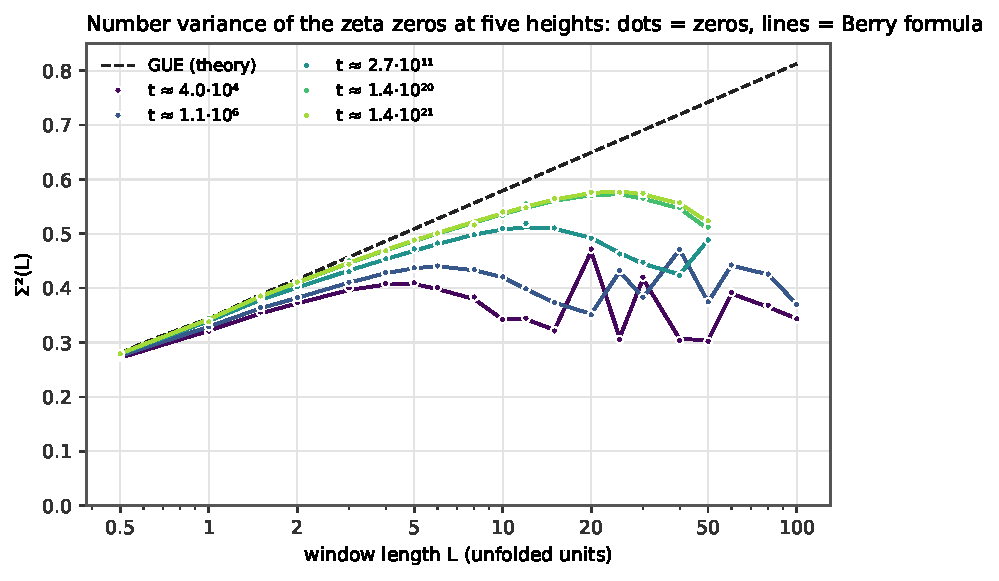
\includegraphics[width=0.92\textwidth]{../figures/01_number_variance_heights_en.pdf}
\caption{Figure 1. Number variance \(\Sigma^2(L)\) of the zeros at five
heights (dots) against Berry's formula (lines, no free parameter) and
GUE (dashed). The oscillations with period \(\approx H/\ln 2\) come from
the prime 2.}
\end{figure}

\hypertarget{the-exact-position-of-the-primes-matters}{%
\subsection{The exact position of the primes
matters}\label{the-exact-position-of-the-primes-matters}}

Berry's formula with Cramér's random primes --- same density
\(1/\ln n\), different positions --- deviates by 5.4--9.9 \% in all
blocks above the lowest ones, i.e.~ten to twenty times more than with
the true primes (Figure 2). The oscillations of \(\Sigma^2(L)\) are
carried by the exact positions of the small primes 2, 3, 5, \ldots{}

\begin{figure}
\centering
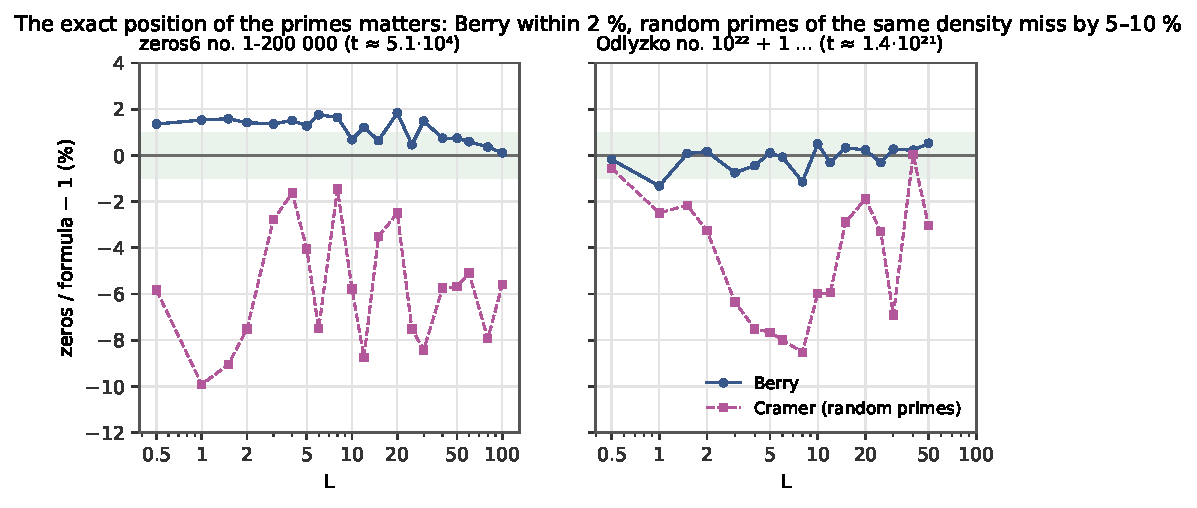
\includegraphics[width=0.92\textwidth]{../figures/02_berry_vs_random_primes_en.pdf}
\caption{Figure 2. Relative deviation of the measured \(\Sigma^2(L)\)
from Berry's formula with the true primes (solid) and with Cramér's
random primes of the same density (dashed); green band \(\pm 1\,\%\).
Left: the lowest block of zeros6; right: Odlyzko's zeros near
\(10^{22}\).}
\end{figure}

\hypertarget{the-saturation-level-grows-with-height}{%
\subsection{The saturation level grows with
height}\label{the-saturation-level-grows-with-height}}

The level of saturation grows from 0.34 (\(t \approx 10^4\)) through
0.40 (\(10^6\)) and 0.46 (\(3\cdot10^{11}\)) to 0.55--0.56
(\(10^{20}\)--\(10^{21}\)), along Berry's curve and below GUE (0.69)
(Figure 3). Unfolding removes the mean density but not the number of
primes below the Heisenberg time,
\(\sum_{p^k < t/2\pi} 1/(k^2 p^k) \sim \ln\ln t\). Hence the statement
``\(\Sigma^2\) in unfolded units does not depend on the height'' holds
for GUE but not for the zeros of \(\zeta\).

\begin{figure}
\centering
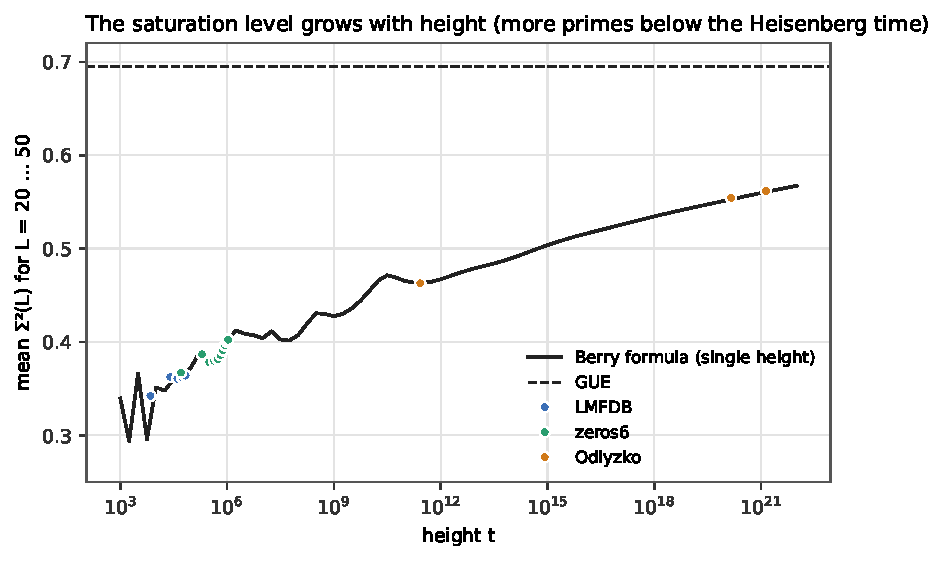
\includegraphics[width=0.92\textwidth]{../figures/03_saturation_level_en.pdf}
\caption{Figure 3. Saturation level (mean \(\Sigma^2\) over
\(L = 20 \dots 50\)) in 18 blocks against height, with Berry's formula
evaluated at a single height (line) and the GUE value (dashed).}
\end{figure}

\hypertarget{spectral-rigidity}{%
\subsection{Spectral rigidity}\label{spectral-rigidity}}

\(\Delta_3\) measured on 800 windows and \(\Delta_3\) computed from
Berry's \(\Sigma^2\) agree within 3.3 \% (mean 1.5 \%; the scatter is
statistical) (Figure 4). At short windows the zeros coincide with GUE
(\(\Delta_3(2) = 0.094\) for both); at long windows they saturate below
GUE: \(\Delta_3(100) = 0.17\) (\(t \approx 10^4\)) to \(0.26\)
(\(t \approx 10^{21}\)) against GUE 0.29 and the crystal value
\(1/12 \approx 0.083\).

\begin{figure}
\centering
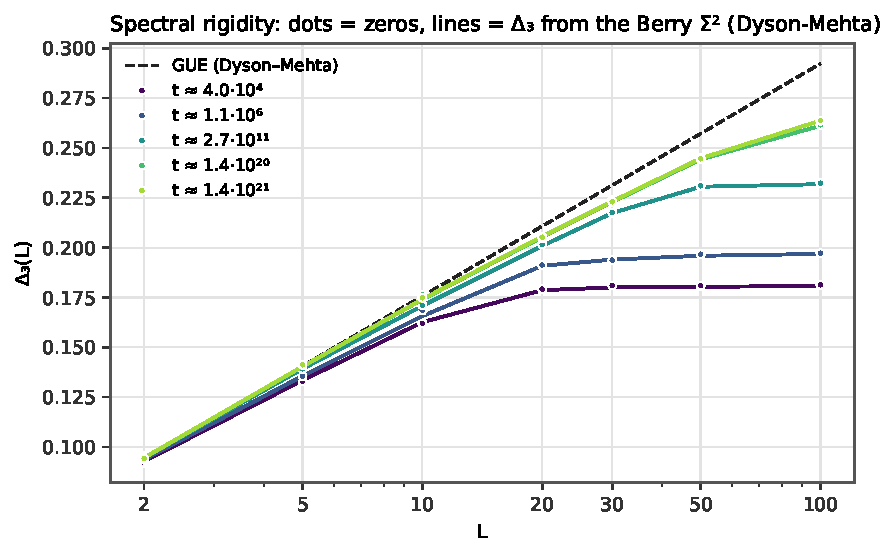
\includegraphics[width=0.92\textwidth]{../figures/04_delta3_en.pdf}
\caption{Figure 4. Spectral rigidity \(\Delta_3(L)\): measured on 800
windows (dots) and computed from Berry's \(\Sigma^2\) through the
Dyson--Mehta relation (lines); GUE dashed.}
\end{figure}

\hypertarget{small-gaps}{%
\subsection{Small gaps}\label{small-gaps}}

The share of unfolded gaps below 0.3 grows from 1.8 \% (first 20,000
zeros) through 2.2 \% (\(10^5\)) and 2.4 \% (\(10^6\)) to 2.6 \%
(\(3\cdot10^{11}\) to \(10^{21}\)), against the GUE value 2.76 \%
(Figure 5). The approach is logarithmically slow, as predicted by the
finite-height corrections of Bogomolny et al.~{[}12{]}.

\begin{figure}
\centering
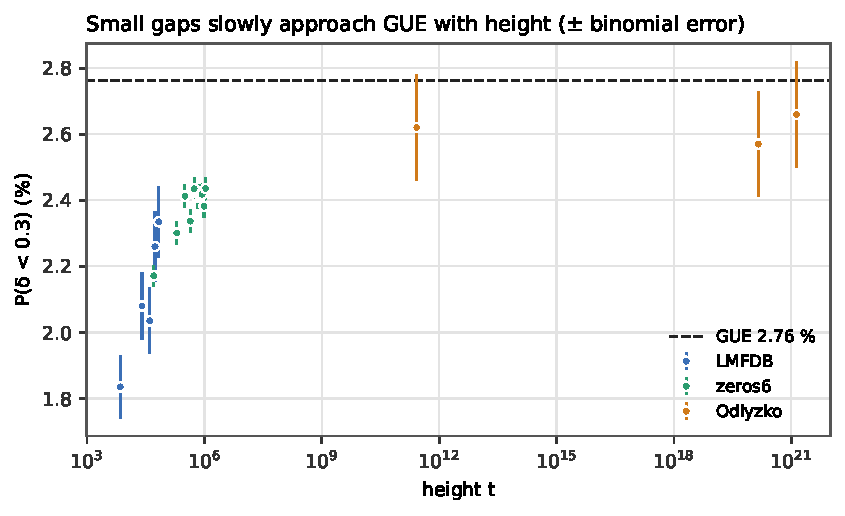
\includegraphics[width=0.92\textwidth]{../figures/05_small_gaps_en.pdf}
\caption{Figure 5. Share of unfolded gaps below 0.3 in each block with
binomial error bars; GUE value dashed.}
\end{figure}

\hypertarget{primes-in-st-at-large-heights}{%
\subsection{\texorpdfstring{Primes in \(S(t)\) at large
heights}{Primes in S(t) at large heights}}\label{primes-in-st-at-large-heights}}

At the zeros no. \(10^{22}+1 \dots 10^{22}+10^4\)
(\(t \approx 1.4\cdot10^{21}\)) the ratio \(a(p)/(-1/\pi\sqrt p)\)
equals 1.007, 1.010, 1.007, 0.996, 0.999, 0.999 for \(p = 2 \dots 13\)
(Figure 6); near \(10^{12}\) and \(10^{21}\) also within 1.2 \%. The
decline of the ratio with \(p\) seen at low heights (up to 12 \% for the
first \(10^4\) zeros) is an effect of sampling \(S(t)\) at the zeros and
disappears with height.

\begin{figure}
\centering
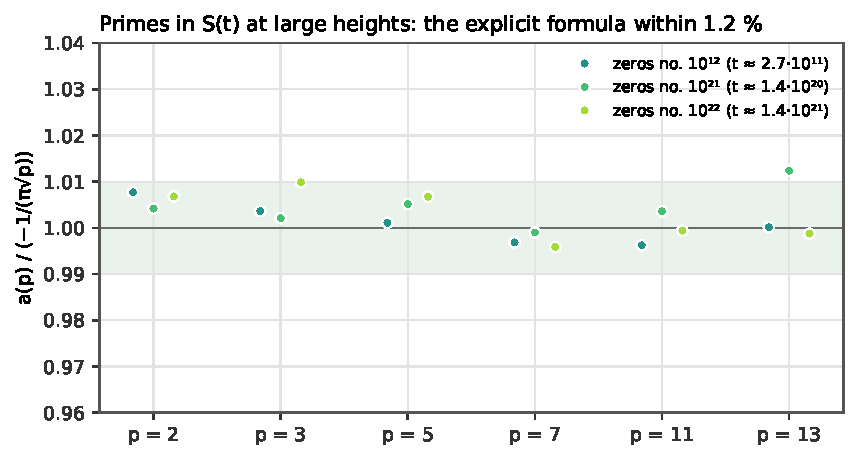
\includegraphics[width=0.92\textwidth]{../figures/06_primes_large_heights_en.pdf}
\caption{Figure 6. Projection of \(S(t)\) on \(\sin(t \ln p)\) divided
by the explicit-formula amplitude \(-1/(\pi\sqrt p)\) at Odlyzko's
heights; green band \(\pm 1\,\%\).}
\end{figure}

\hypertarget{the-crossover-scale}{%
\subsection{The crossover scale}\label{the-crossover-scale}}

Defining the departure from GUE as the smallest \(L^*\) at which the
zeros lie 5 \% (10 \%) below GUE gives \(L^* \approx 0.09\)--\(0.15\,H\)
(\(0.21\)--\(0.37\,H\)), from \(L^* = 0.67\) at \(H = 7\) to
\(L^* = 6.0\) at \(H = 46.8\), equal to the value from Berry's formula
(Figure 7). The transition is a smooth crossover whose scale grows with
the Heisenberg time \(\ln(t/2\pi)\), not a sharp threshold; the
threshold itself (5 \% or 10 \%) changes \(L^*\) by a factor of about
three.

\begin{figure}
\centering
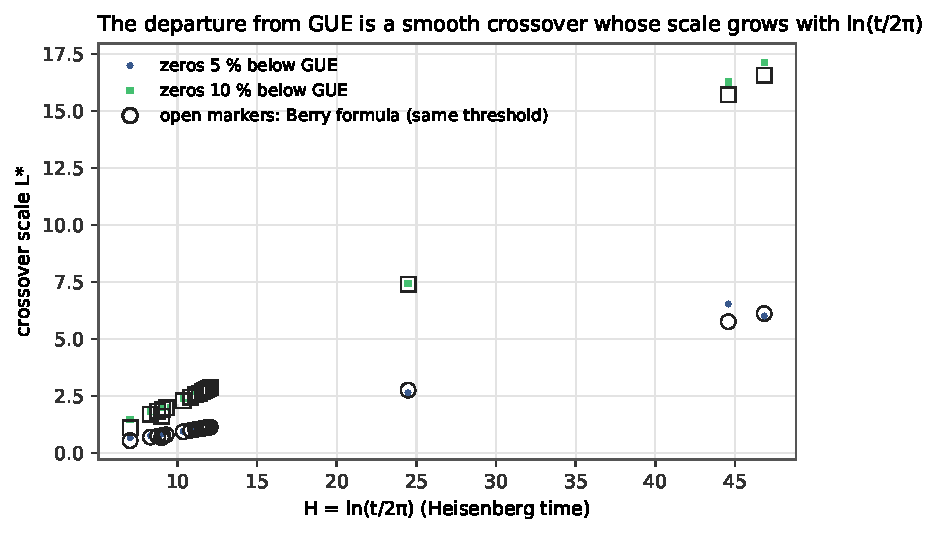
\includegraphics[width=0.92\textwidth]{../figures/07_crossover_scale_en.pdf}
\caption{Figure 7. Crossover scale \(L^*\) at which the zeros fall 5 \%
(circles) or 10 \% (squares) below GUE, against \(H = \ln(t/2\pi)\);
open markers: the same threshold applied to Berry's formula.}
\end{figure}

\hypertarget{sieve-for-candidate-spectra}{%
\subsection{Sieve for candidate
spectra}\label{sieve-for-candidate-spectra}}

\begin{center}\small
\begin{tabular}{@{}lcccc@{}}
\toprule
candidate (20,000 levels) & density & GUE gaps & primes & saturation \\
\midrule
true zeros & pass & pass & pass & pass \\
levels $xp$ (Berry--Keating) & pass & fail & fail & pass \\
$xp$ + prime orbits $p^k \le 997$ & pass & pass & pass & pass \\
GUE matrix & pass & pass & fail & fail \\
GOE matrix & pass & fail & fail & fail \\
Poisson & fail & fail & fail & fail \\
zeros + noise $\sigma = 0.3$ & pass & fail & fail & pass \\
\bottomrule
\end{tabular}
\end{center}

A GUE random matrix reproduces the local statistics but has no prime
content and no saturation. The levels of \(xp\) completed by the prime
orbits of the explicit formula pass all four stages --- a construction
that shows what an operator would have to contain, not an operator. The
zeros of twelve Dirichlet \(L\)-functions \(L(s, \chi_q)\),
\(q = 3 \dots 41\), pass with the weights \(\chi(p)\), and the sign of
\(a(p)\) equals \(\chi(p)\) in 67 of 67 pairs: the signal is the
arithmetic of the particular function.

\hypertarget{discussion}{%
\section{Discussion}\label{discussion}}

Berry's formula is the diagonal approximation of the explicit (trace)
formula; its success over 17 orders of magnitude in height, without a
free parameter, confirms that the long-range statistics of the zeros are
fixed by the primes. The residual of about 1 \% in the lowest blocks is
consistent with the expected size of the off-diagonal
(Hardy--Littlewood) corrections computed by Bogomolny and Keating
{[}8{]} together with finite-sample noise; separating the two is the
subject of follow-up work. The saturation and the other statistics
follow from the arithmetic of the primes, not from the position of the
zeros: they neither confirm nor refute the Riemann hypothesis, and no
self-adjoint operator with this spectrum is known (Hilbert--Pólya
remains open). Berry compared his formula with Odlyzko's zeros near
\(10^{12}\) in 1988; the present study repeats that comparison and
extends it to \(10^{21}\), \(10^{22}\) and two million low zeros with
independent checks.

\hypertarget{reproducibility}{%
\section{Reproducibility}\label{reproducibility}}

The script \texttt{compute\_rigidity.py} recomputes every number of
Sections 4.1--4.7 from the original text files of zeros (LMFDB,
Odlyzko), and \texttt{figures.py} draws every figure from its output.
The script \texttt{independent\_check.py} recomputes the same quantities
with partly different algorithms (primes by a segmented sieve, the prime
tail above \(10^6\) and \(\Delta_3\) from Berry's \(\Sigma^2\) by
quadrature) and agrees within \(10^{-11}\). The results of the sieve
(Section 4.8) are given as data. The computations were developed and
verified in the protected MAYAN ALFA V1008 laboratory (internal, version
34.47; mayanalfa.com), which is not part of this package. The package
lists the SHA-256 hash of every file. Text, figures and data are
released under the Creative Commons Attribution 4.0 International
licence (CC BY 4.0); the scripts under the MIT licence.

\hypertarget{references}{%
\section*{References}\label{references}}

\begin{enumerate}
\def\labelenumi{\arabic{enumi}.}
\tightlist
\item
  Montgomery, H. L. (1973). The pair correlation of zeros of the zeta
  function. Proc. Symp. Pure Math. 24, 181--193.
\item
  Berry, M. V. (1985). Semiclassical theory of spectral rigidity. Proc.
  R. Soc. A 400, 229--251.
\item
  Berry, M. V. (1988). Semiclassical formula for the number variance of
  the Riemann zeros. Nonlinearity 1, 399--407.
\item
  Odlyzko, A. M. (1987). On the distribution of spacings between zeros
  of the zeta function. Math. Comp. 48, 273--308.
\item
  Dyson, F. J. \& Mehta, M. L. (1963). Statistical theory of the energy
  levels of complex systems. IV. J. Math. Phys. 4, 701--712.
\item
  Mehta, M. L. (2004). Random Matrices, 3rd ed.~Academic Press.
\item
  Berry, M. V. \& Keating, J. P. (1999). The Riemann zeros and
  eigenvalue asymptotics. SIAM Rev.~41, 236--266.
\item
  Bogomolny, E. B. \& Keating, J. P. (1996). Gutzwiller's trace formula
  and spectral statistics: beyond the diagonal approximation. Phys.
  Rev.~Lett. 77, 1472--1475.
\item
  Gonek, S. M., Hughes, C. P. \& Keating, J. P. (2007). A hybrid
  Euler--Hadamard product for the Riemann zeta function. Duke Math. J.
  136, 507--549.
\item
  Dumitriu, I. \& Edelman, A. (2002). Matrix models for beta ensembles.
  J. Math. Phys. 43, 5830--5847.
\item
  The LMFDB Collaboration. The L-functions and Modular Forms Database.
  \url{https://www.lmfdb.org/}
\item
  Bogomolny, E., Bohigas, O., Leboeuf, P. \& Monastra, A. G. (2006). On
  the spacing distribution of the Riemann zeros: corrections to the
  asymptotic result. J. Phys. A 39, 10743--10754.
\item
  Odlyzko, A. M. Tables of zeros of the Riemann zeta function.
  \url{https://www-users.cse.umn.edu/~odlyzko/zeta_tables/}
\end{enumerate}

\end{document}
